\chapter{Mechanisms Controlling the Land/Sea Contrast} 


\label{mechanisms} 

\lhead{Chapter 4. \emph{Mechanisms}} 

\section{Introduction}
\paragraph{Discuss GW theories, relevance to interannual var.}

%----------------------------------------------------------------------------------------
%	influence of SSTs on Continental temps
%----------------------------------------------------------------------------------------

\section{The Influence of Tropical Oceans on Land}

\paragraph{Strong land/ocean connection in tropics}
When looking at the relationship between $T_{land}$ and SSTs there is an 
assymetry between the response of $T_{land}$ to tropical and extra-tropical SST 
forcing. We investigate this assymetry and the importance of the tropical oceans 
in regulating regional and global land surface temperatures using modelling 
experiments. In the 1K experiments a constant +/-1K SST anomaly is applied to 
tropical or extra-tropical regions, in the Half-AMIP experiments the same 
regional restrictions are used but instead of a constant forcing, variability is 
imposed using observed SST anomalies. The Pacemaker experiments are forced with 
an idealised ENSO in the tropical Pacific and a slab ocean or fixed SSTs 
elsewhere.

\subsection{1K Experiments}

Figure \ref{fig:1K} shows the surface temperature response (control removed) 
from the 1K experiments; where 1K was added to the oceans in the tropics, 
extra-tropics or globally. In response to a tropical SST perturbation there is a 
large tropical response, greatest over equatorial South America and Africa, 
India and the maritime continent (Fig.\ref{fig:1K} a). The tropical 1K ocean 
perturbation leads to $T_{land}>+1$K in most tropical areas. Thus the SST 
forcing is amplified. The extra-tropical land the response to the tropical 
forcing is not significant everywhere, but some regions also show an amplified 
response to the tropical SST forcing (e.g. central Asia and parts of Europe and 
North America).  An extra-tropical $T_{land}$ response to tropical SSTs is seen 
for seasonal averages in the winter months of each hemisphere, the Northen 
Hemsiphere winter response is shown in Figure \ref{fig:1K} e.

When looking at the annual mean response of $T_{land}$ to extra-tropical SST 
perturbations there is little significant response, however for seasonal 
averages both hemispheres show a significant response in their respective winter 
months, shown for the Northern Hemisphere in Figure \ref{fig:1K} e-g. The 
response of $T_{land}$ is also amplified in some regions relative to the initial 
perturbation.  However, the extra-tropical forcing again leads to a weaker land 
response than the tropical forcing, as was also found in the AMIP simulations.  
Also similar to the AMIP simulations we again find that the  global SST forcing 
has a bigger impact than the tropical only forcing for the annual mean. In 
addition the response of the global SST forcing is greater than the 
superposition of the tropical and extra-tropical forcing (comparing 
Fig.\ref{fig:1K} c and d).  This again indirectly suggests that the 
extra-tropical SST forcing does lead to a significant land response.

\begin{figure}[ht]
	\centering
	\includegraphics[width=0.45\textwidth]{{meantemp.trop}.eps}
	\includegraphics[width=0.45\textwidth]{{meantemp.trop.DJF}.eps}\\
\vspace{-0.9cm}
	\includegraphics[width=0.45\textwidth]{{meantemp.extr}.eps}
	\includegraphics[width=0.45\textwidth]{{meantemp.extr.DJF}.eps}\\
\vspace{-0.9cm}
	\includegraphics[width=0.45\textwidth]{{meantemp.glob}.eps}
	\includegraphics[width=0.45\textwidth]{{meantemp.glob.DJF}.eps}\\
\vspace{-0.5cm}
	\includegraphics[width=0.45\textwidth]{{meantemp.addt}.eps}
	\includegraphics[width=0.45\textwidth]{{meantemp.addt.DJF}.eps}\\
\caption{Mean $T_{surf}$ response for sensitivity experiments  a) 1K added to 
	tropical oceans b) 1K added to extra-tropical oceans c) 1K added to global 
	oceans d) Combined response of tropical 1K oceans plus extra-tropical 1K 
	ocean. Masked at 95\% confidence levels.}
\label{fig:1K}
\end{figure}



\subsection{Half-AMIP Experiments}

In Figure \ref{fig:ftest} f-tests are used to measure the increase in annual 
temperature variability due to SST variability at the surface and at the 300hPa 
pressure level relative to a simulation with fixed SST climatology. Figure  
\ref{fig:ftest} a) and d) show that global SST variability has a substantial 
impact on the tropical atmospheric and surface temperature variability. In the 
extra-tropical regions the impact is much weaker, but still statistically 
significant in some regions.

In order to separate the influence of the tropical SST variability from that of 
the extra-tropical SST, we repeat the AMIP experiment forced with the historical 
SST variability just in the tropics or just in the extra-tropical regions. The 
impact of the tropical-only SST variability is similar to the global SST 
variability, with a clear and strong impact in the tropical regions.  The AMIP 
simulation with extra-tropical-only SST variability has only a very weak to no 
impact on the regional (grid-box scale) atmospheric and surface temperature 
variability.  However, if we compare the global AMIP versus the tropical only 
AMIP run we still can see a somewhat larger increase in variance over land in 
the global AMIP run. This indirectly suggests that the extra-tropical SST 
forcing does play a role, although it is much smaller than the tropical forcing.  
In summary the AMIP experiments suggest a clear tropical SST forcing to the 
atmospheric and land surface temperatures, but a much weaker or no forcing from 
the extra-tropical SST.

\begin{figure}[ht]
	\includegraphics[width=1.0\textwidth, trim={8.5cm 5cm 11cm 
	1cm},clip=true]{{ftest_sub_sfc}.pdf}
	%\vspace{-1.8cm}
	\includegraphics[width=1.0\textwidth, trim={8.5cm 5cm 11cm 
	1cm},clip=true]{{ftest_sub_300}.pdf}
	\caption{F-test of annual mean temperature for AMIP-type runs. Surface 
		temperature response on top row, 300hPa response on bottom row.	a),d) AMIP 
		run with detrended HadISST used globally b),e) AMIP-type run with detrended 
		HadISST in extra-tropics, climatological SSTs elsewhere c),f) AMIP-type run 
		with detrended HadISST in tropics, climatological SSTs elsewhere tropics.  
		All values masked at 90\% confidence levels. Hatching indicates areas of 
	ocean with SST variability.}
	\label{fig:ftest}
\end{figure}

\subsection{Tropical Troposphere}
The Half-AMIP experiments demonstrate an important process in the strong 
tropical land/ocean connection. Figures \ref{fig:ftest} d)--e) show the value of 
an f-test on the 300hPa surface, measuring the increase (values above zero) in 
temperature variability due to imposed SST variability. The results for global 
and tropical AMIP runs are very similar, with the global AMIP having slightly 
higher values in the tropics and some more variability in the extratropics, 
whereas there's no significant tropospheric response to extra-tropical SSTs.  
The tropospheric response in the tropics can be described with two key 
processes; the large amplitude of the temperature variability is due to latent 
heating by deep moist convection, and the -- largely -- zonally uniform pattern 
is the result of the tropical free troposphere not being able to maintain 
horizontal pressure gradients due the small coriolis number (REF). This results 
in tropical SST perturbations being amplified in the troposphere and efficiently 
transported over tropical land. The area with the largest tropospheric anomalies 
is over the eastern tropical pacific, the ENSO region. ENSO is the dominant 
driver of interannual temperature variability and while the ENSO induced 
tropospheric anomalies are distributed around the tropics, there is still a 
maximum in that area. The role of ENSO is further explored with the Pacemaker 
experiments.


%----------------------------------------------------------------------------------------
%	ENSO
%----------------------------------------------------------------------------------------

\subsection{Pacemaker Experiments}


On inter-annual timescales ENSO is the most significant global climate driver. 
It is therefore remarkable that in the analysis of the CMIP5 model simulations 
the NINO3 region did not show up with a high correlation to global $T_{land}$ 
(see Fig.\ref{fig:cmip_cormap}). The ENSO region in the tropical Pacific has a 
lower correlation with $T_{land}$ than adjacent regions and the other ocean 
basins. Using the combined monthly mean CMIP5 surface temperature anomalies, 
Fig.\ref{fig:xcor} e) shows the lagged correlations between NINO3 SST and global 
$T_{land}$. The NINO3 region is seen to lead global land by 4 months.  Typically 
land has a fast response time to forcings, which would not result in a 
4 month delay, so this result suggests that the full land response is not 
directly forced by the NINO3 SST but is most likely caused by something else. 
This other forcing may be delayed to the ENSO variability by about 4 months. 
Since we have seen in Fig.\ref{fig:cmip_cormap} that global $T_{land}$ is highly 
correlated to other tropical ocean SST, it seems likely that $T_{land}$ is 
linked to the slower ocean response in the remote tropical oceans and not 
directly to the NINO3 region.

To address this question we conducted a series of idealised ENSO-response 
experiments. In the first experiment we prescribe an oscillating ENSO pattern (a 
regression between NINO3 and SSTs shown in Fig.\ref{fig:regpat}) in the tropical 
Pacific and a fixed 12 month climatology of SSTs elsewhere.  The oscillation 
period of the ENSO signal is 4 years, peaking in January. In the second 
experiment we allow SST variability outside the tropical Pacific simulated by a 
simple slab ocean model with a mixed layer depth of 50 metres.  Thus, in the 
second experiment the global ocean SSTs can respond to the oscillating ENSO 
pattern forcing.

\begin{figure}[ht]
	\includegraphics[width=\textwidth]{{regpat}.eps}\\
	\caption{Pattern used in ENSO experiments. Result of regression between NINO3 
	and global SST.}
	\label{fig:regpat}
\end{figure}

Figure \ref{fig:xcor} (i-l) shows cross-correlations from the ENSO-FIXSST and 
ENSO-Slab forcing experiments. In i) and j) we see that for the fixed SST 
experiment the global and tropical land responds to the ENSO-like forcing (red 
line), and does so without the delay seen in Figure \ref{fig:xcor} e). When a 
slab ocean is introduced the land responds with a realistic delay of around 4 
months.  The peak slab ocean response is at 6 months, implying that the land is 
responding immediately to the initial Pacific ocean forcing and then 
subsequently to the delayed slab ocean response. The delayed land response is 
also associated with a higher correlation to the NINO3 region. Comparing the 
global and tropical averages, the main difference is the magnitude of the peak 
correlation, but in the tropics the slab ocean also results in the peak land 
correlation being higher than the peak ocean correlation. So the delayed 
response of the remote tropical oceans to a Pacific ocean forcing explains both 
the delayed land response and some part of the amplification of the oceanic 
temperature signal over land. In the extra-tropics there is only a very weak 
influence of the ENSO forcing on land temperatures in the sensitivity 
experiments (Fig.  \ref{fig:xcor} g, h), and the tropical Pacific has little 
influence on the slab ocean in the extra-tropics. The observations and CMIP5 
models also don't show a significant relationship between the extra-tropics and 
NINO3 (Fig.\ref{fig:xcor} g,h,k,l).

\clearpage
\begin{figure}[ht]
	\includegraphics[width=\textwidth, trim={5cm -1cm 5cm 
	-0.5cm},clip=true]{{xcor_sub_obs}.eps}
	\includegraphics[width=\textwidth, trim={5cm -1cm 5cm 
	-0.5cm},clip=true]{{xcor_sub_cmip5}.eps}
	\includegraphics[width=\textwidth, trim={5cm -1cm 5cm 
	-0.5cm},clip=true]{{xcor_sub_enso}.eps}
\caption{Cross-correlations between the NINO3 region and land and ocean.  
	Observations (top row), combined CMIP5 models (middle row), Two sensitivity 
	experiments (bottom row);  Atmospheric model forced with ENSO-like oscillation 
	in tropical Pacific and fixed SSTs elsewhere (red line), slab ocean elsewhere 
	(green, blue lines).  Global land and ocean (a,e,i), tropical land and ocean 
	(b,f,j), NH extra-tropical land and ocean (c,g,k) and SH extra-tropical land 
	and ocean (d,h,l).  NINO3 autocorrelation included for reference (black dashed 
line).}
	\label{fig:xcor}
\end{figure}

To summarise thus far; we see that tropical SSTs strongly influence tropical and 
- to a lesser extent - extra-tropical continental temperatures; SST anomalies 
are amplified in the tropical troposphere and efficiently transported over land; 
ENSO is the dominant source of interannual variability and can influence land 
surface temperatures via the troposphere. However we now wish to investigate the 
process by which SST variability leads to amplified $T_{land}$ variability.  

% \section{ENSO}
% \begin{itemize}
% 	\item ENSO is source of tropical inter-annual variability.
% 	\item Temperature anomaly seen throughout tropical troposphere
% 	\item Land responds quickly - within a month - to initial anomaly.
% 	\item Remote tropical oceans response is delayed by 3-4 months.
% 	\item Timing of delay of remote tropical oceans is a function of mixed layer 
% 		depth.
% 	\item Land responds to the delayed forcing by remote trop oceans.
% 	\item Mean land response appears to be delayed, i.e. when plotted with lag 
% 		correlations.
% 	\item Delayed land response is linear combination of initial response to 
% 		Pacific ocean and response to delayed remote tropical oceans.
% 	\item Land response is amplified due to previously discussed process.
% 	\item The land response is further amplified by secondary response to remote 
% 		tropics.
% \end{itemize}


%----------------------------------------------------------------------------------------
%	LAPSE RATE
%----------------------------------------------------------------------------------------

\section{The Lapse Rate Mechanism}

We are now going to investigate the relationship between tropospheric anomalies 
and the surface by looking at the warming lapse rate mechanism described by 
\citet{Joshi2007} and \citet{Byrne2013a}, and testing it's validity for 
interannual variability. 

We first take a look at the vertical structure of the relationship between land 
and ocean temperatures comparing the Pacemaker experiment with a climatology run 
(i.e. no SST variability).  Using tropical averages, Figure 
\ref{fig:linreg_plev} shows regression values for the $T_{tropos}$ at different 
pressure levels as a function of the surface temperature $T_{land}$ (a) and 
$T_{ocean}$ (b), with the green line for the column of air above tropical land, 
blue for the column of air above tropical ocean, and the black line is the 
column above the remote tropical ocean, essentially the tropical oceans with the 
area of forcing removed.  Looking first at Figure \ref{fig:linreg_plev} a), in 
the simulation without any SST variability (dashed lines) the higher level 
tropical temperatures over land areas are not related to $T_{land}$ as the 
regression values between the surface and tropospheric temperatures falls to 
zero above \SI{800}{\hecto\pascal}, indicating that the atmospheric internal 
$T_{land}$ variability (independent of SST variability) is limited to the near 
surface layers and is not strongly related to the upper free $T_{tropos}$. In 
the simulation with SST variability the tropospheric temperature shows a strong 
relationship with the surface $T_{land}$ variability at all levels. 

Now focusing on Figure \ref{fig:linreg_plev} b), a distinctive feature for the 
troposphere above oceans (blue line) is the large increase in the regression 
values in the upper troposphere. This is a well known signature of moist
convection; a \SI{1}{\kelvin} anomaly at the surface corresponds to a 
\SI{2}{\kelvin} anomaly in the upper level temperatures, due to the latent heat 
release by moist convection (\citet{Joshi2007}, \citet{Byrne2013}, 
\citet{Dommenget2009}, etc.). The anomalies above land regions don't reach the 
same peak in the upper troposphere, however in the middle troposphere, around 
the \SI{700}{\hecto\pascal} to \SI{500}{\hecto\pascal} level, the two lines 
coincide, similar to the level in the atmosphere described by \citet{Joshi2007} 
where there is no land/ocean warming contrast. It's in the levels below 
\SI{800}{\hecto\pascal} where the variability increases above land. This figure 
would indicate a value of $R_{l/o}$ of around 1.2, as for a \SI{1}{\kelvin} 
anomaly of $T_{ocean}$ we have a \SI{1.2}{\kelvin} response in $T_{land}$.  

An advantage of the Pacemaker experimental design is that the area of ocean 
forcing is very well constrained. When looking at the response to an ENSO 
forcing from the tropical Pacific, the remote tropical oceans will also have 
their own, potentially considerable, internal variabiltiy due to ocean dynamics.  
In the Pacemaker experiment the remote -- slab -- oceans have no dynamics. In 
this way we can consider the Pacific Ocean forcing as an external forcing, and 
measure the seperate response of land and ocean. In Figure \ref{fig:linreg_plev} 
b) the black line is such a measurement, the only variability for this region is 
imposed via the Pacific ocean forcing.  The remote tropical response is similar 
to the land response in shape; it also lacks the large amplification in the 
upper troposphere indicating that the upper levels are responding to the Pacific 
forcing and not being driven by moist convection.  At all levels the remote 
tropical response is less than the land response which means there is no clear 
level where there is no land/ocean contrast however the two lines diverge more 
near the surface, with the largest difference in gradients below 
\SI{800}{\hecto\pascal}. In the global warming lapse rate theory, the increased 
continental lapse rate is due to reduced moisture availability and thus lower 
relative humidities. The vertical structure above land and ocean is further 
explored with a one and two-dimensional model.


\begin{figure}[ht]
		\includegraphics[width=0.45\textwidth]{{linreg_land_profile}.eps}
		\includegraphics[width=0.45\textwidth]{{linreg_ocean_sans_profile}.eps}\\
	\caption{Linear regression coefficients for temperature above tropical land 
	and ocean as linear model of a) $T_{land}$ (1000hPa surface) and b) 
$T_{ocean}$, for forced run (solid) and control run (dashed). i.e.  
$T_{plv,land} = a T_{sfc,land} + b$, and $T_{plv,ocean} = a T_{sfc,land} + b$}
\label{fig:linreg_plev}
\end{figure}


\subsection{The Weak Temperature Gradient Approximation}
As previously mentioned the tropical troposphere is unable to maintain strong 
temperature gradients. Near the equator the small Coriolis parameter results in 
geostrophic adjustments by gravity waves and Kelvin waves that remove horizontal 
temperature gradients.  In the extra-tropics the quasi-geostrophic approximation 
gives a simplified dynamical model, based on the balance of the pressure 
gradient force and rotation.  The WTG approximation is analagous and uses the 
small horizontal temperature and pressure gradients as a constraint on the 
large-scale flow and diabatic processes. The temperature equation can be 
simplified to give a balance between diabatic heating and vertical advection 
\ref{Sobel2001}. The usefulness of the WTG approximation doesn't quite match 
that of quasi-geostrophy due to the importance in the tropics of deep 
convection, which has it's own parameterization difficulties, but the WTG 
approximation does allow for the parameterization of large-scale dynamics. It is 
in this context that the WTG approximation is used in this study, as it allows 
us to model the land/ocean contrast using a single column model. Temperature 
profiles can be generated in a column above ocean, then those profile can be 
imposed above a land surface. The temperature profile is constant in the free 
troposphere and allowed to vary near the surface, thereby simulating the control 
of the free tropospheric temperatures by (for example) Pacific ocean anomalies.


\subsection{Experiments with a Single-Column Model}
\label{sec:mech_scm}
We are interested in the land temperature response to a tropospheric forcing, a 
single column model allows us to vary parameters controlling land surface 
properties while keeping the forcing stable. We begin by generating the 
temperature profiles above an ocean column with prescribed SSTs. As the focus is 
interannual variabilty an SST value of \SI{26}{\degreeCelsius} was used as the 
mean profile, then for the variability the SSTs were varied by either fractions 
of a degree, to simulate the magnitude of interannual anomalies, or by many 
degrees to clearly show the mean response.

The tropospheric response is shown in Figure \ref{fig:scmsstprof}. In 
Fig.\ref{fig:scmsstprof} a) the temperature anomalies relative to 
\SI{26}{\degreeCelsius} show the increase with height of both positive and 
negative SST anomalies.  The magnitude is more clearly shown in 
Fig.\ref{fig:scmsstprof} b), which measures the amplification of the SST anomaly 
with height. For example, a value of 2 at \SI{300}{\hecto\pascal} indicates that 
an anomoly of \SI{2}{\kelvin} would lead to a \SI{4}{\kelvin} anomaly at that 
height.  It shows that positive and negative anomalies are amplified to a 
similar extant, although the tropopause is higher for the positive anomalies 
leading to a discrepency around \SI{200}{\hecto\pascal}. Figure 
\ref{fig:scmsstprof} c) demonstrates that the upper tropospheric anomalies are a 
result of heating by moist convection.


\begin{figure}[ht]
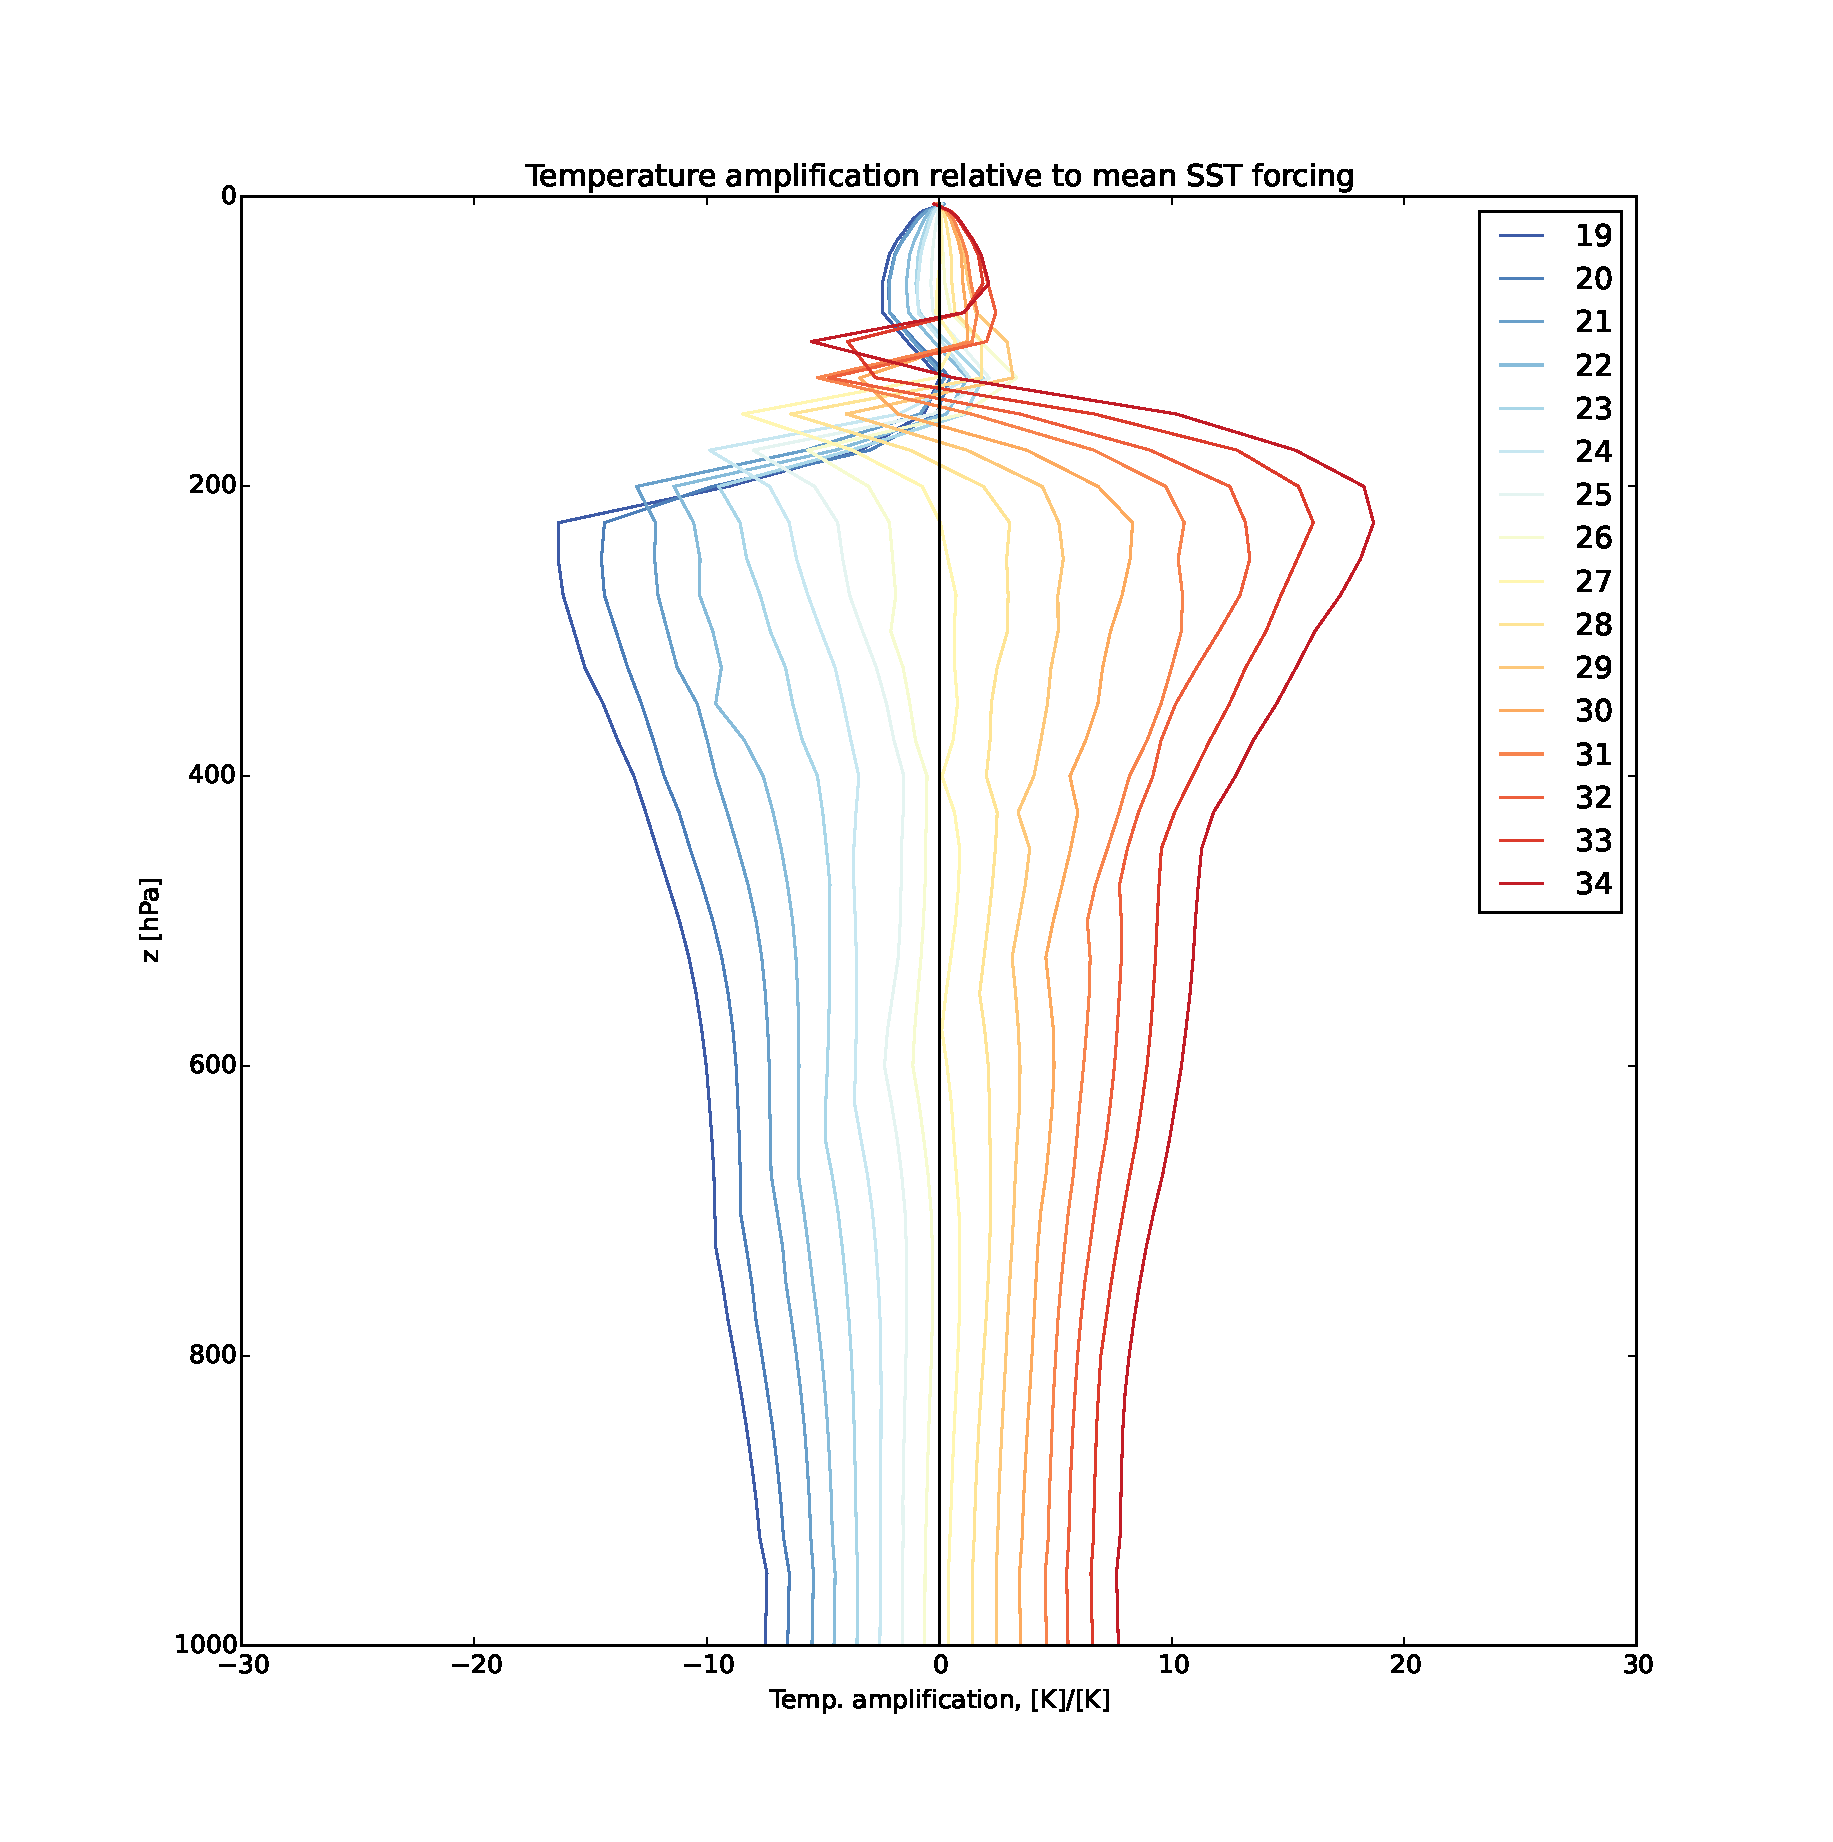
\includegraphics[width=0.3\textwidth]{enso_prof_temp_mean.eps}
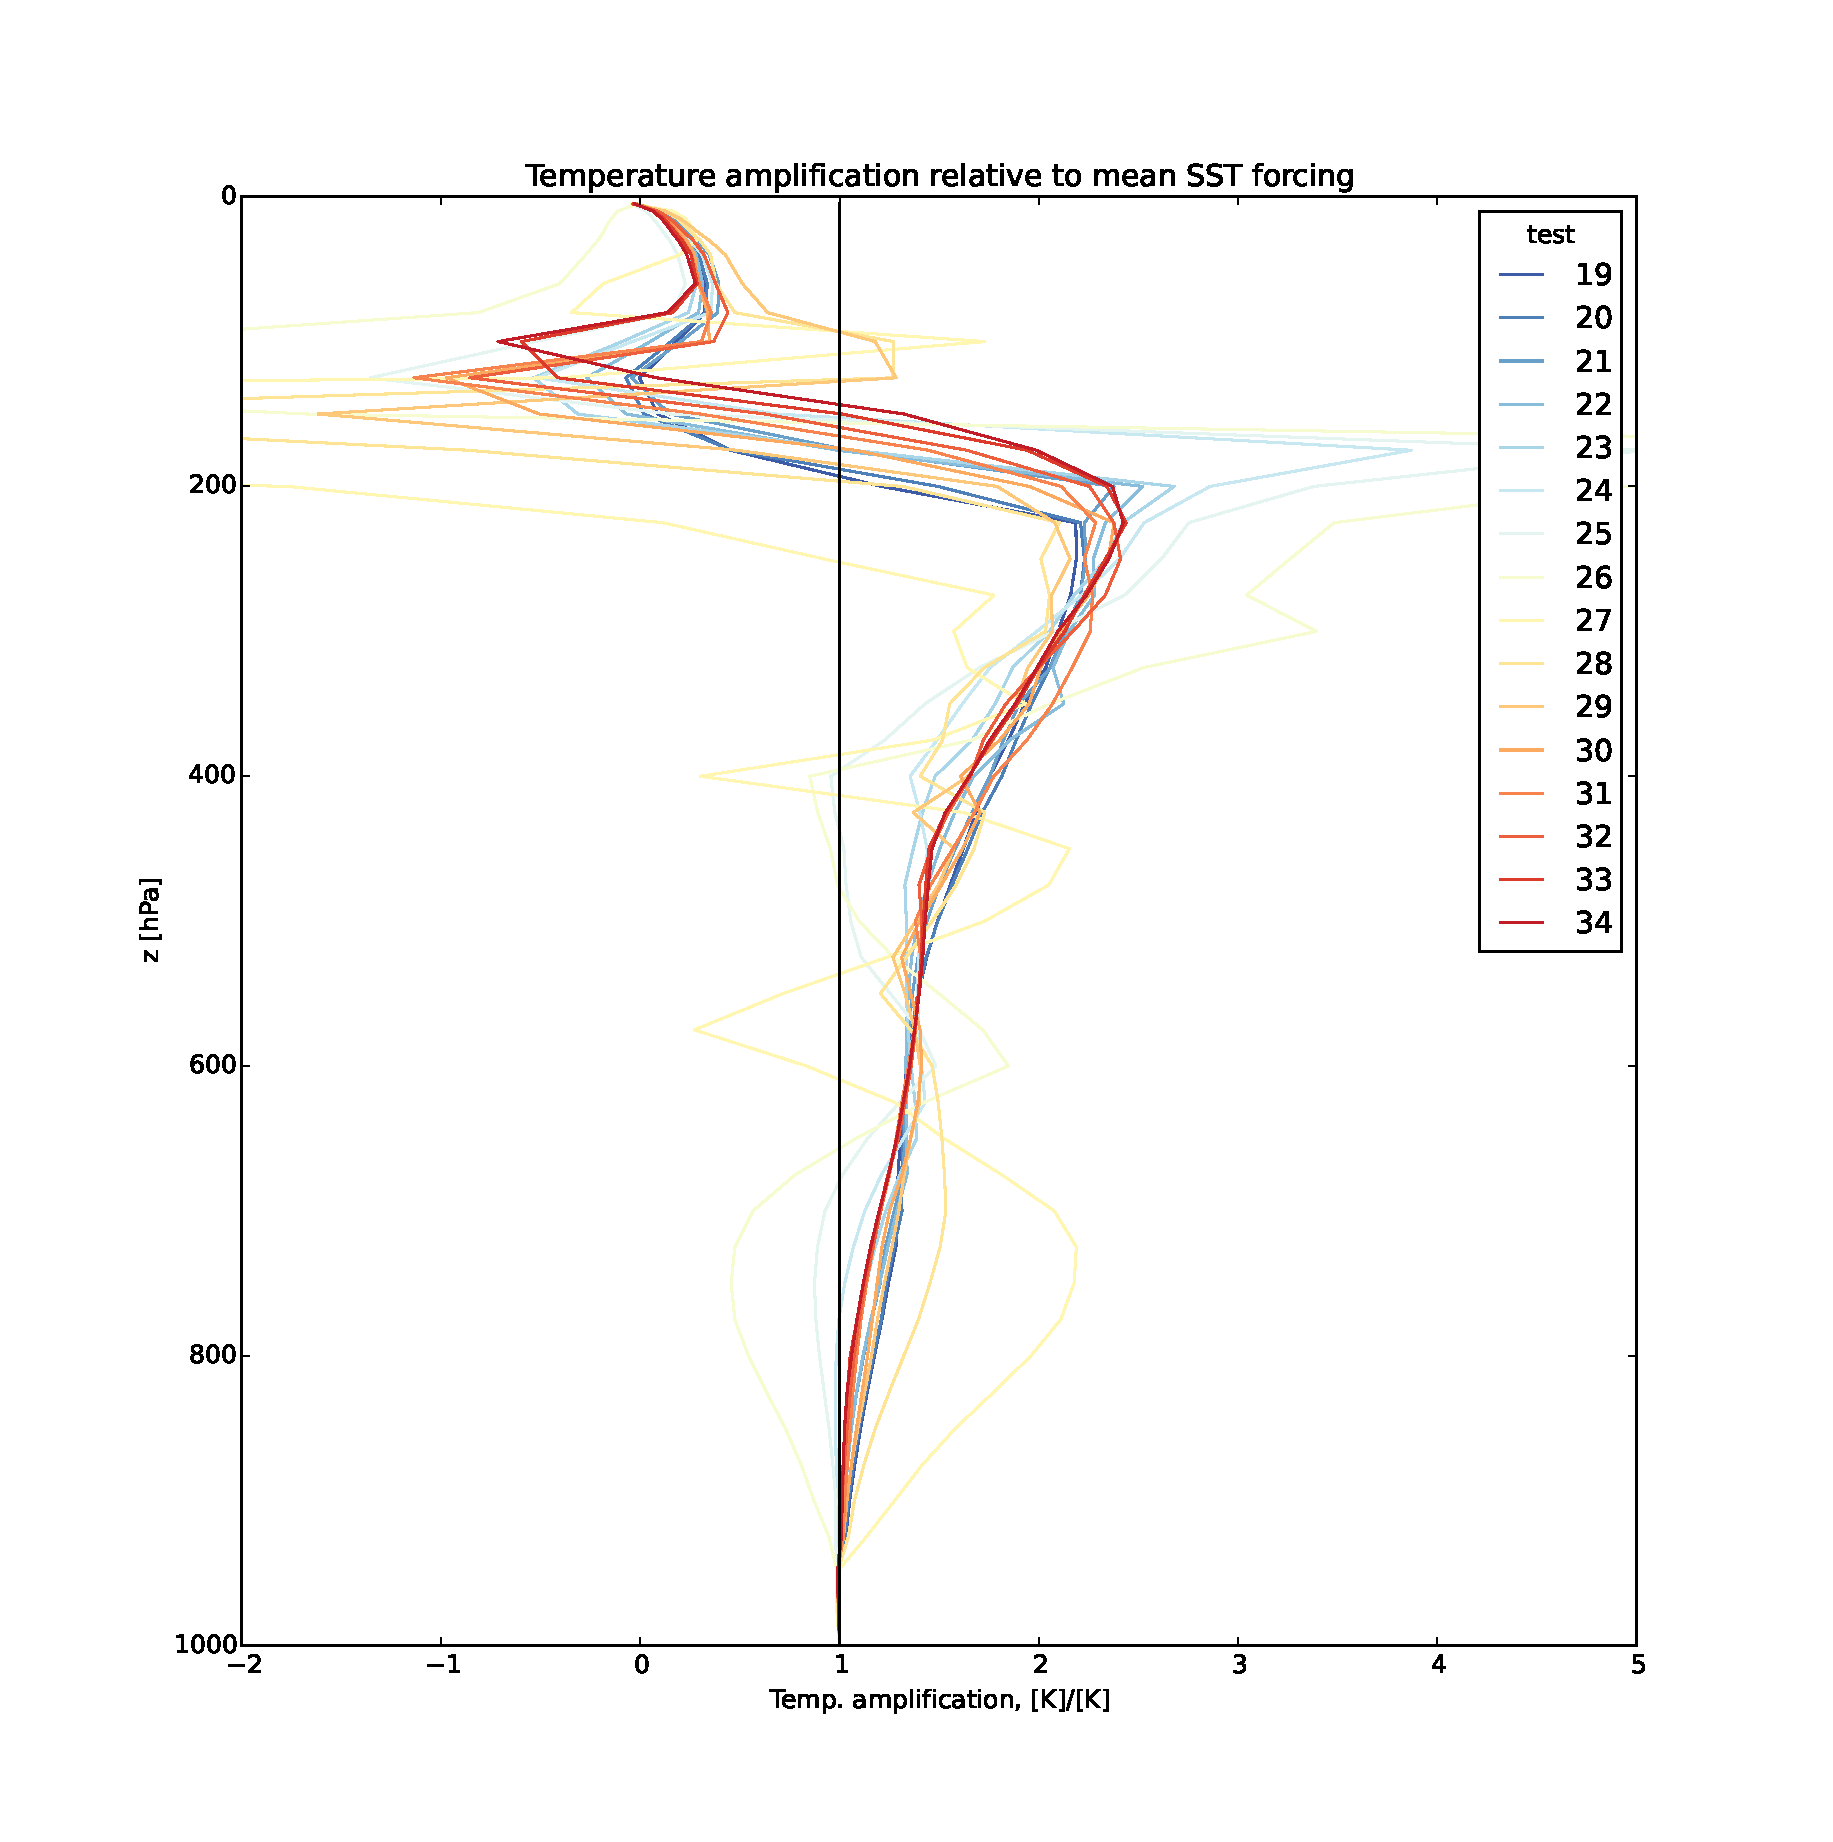
\includegraphics[width=0.3\textwidth]{enso_prof_ampratio_mean.eps}
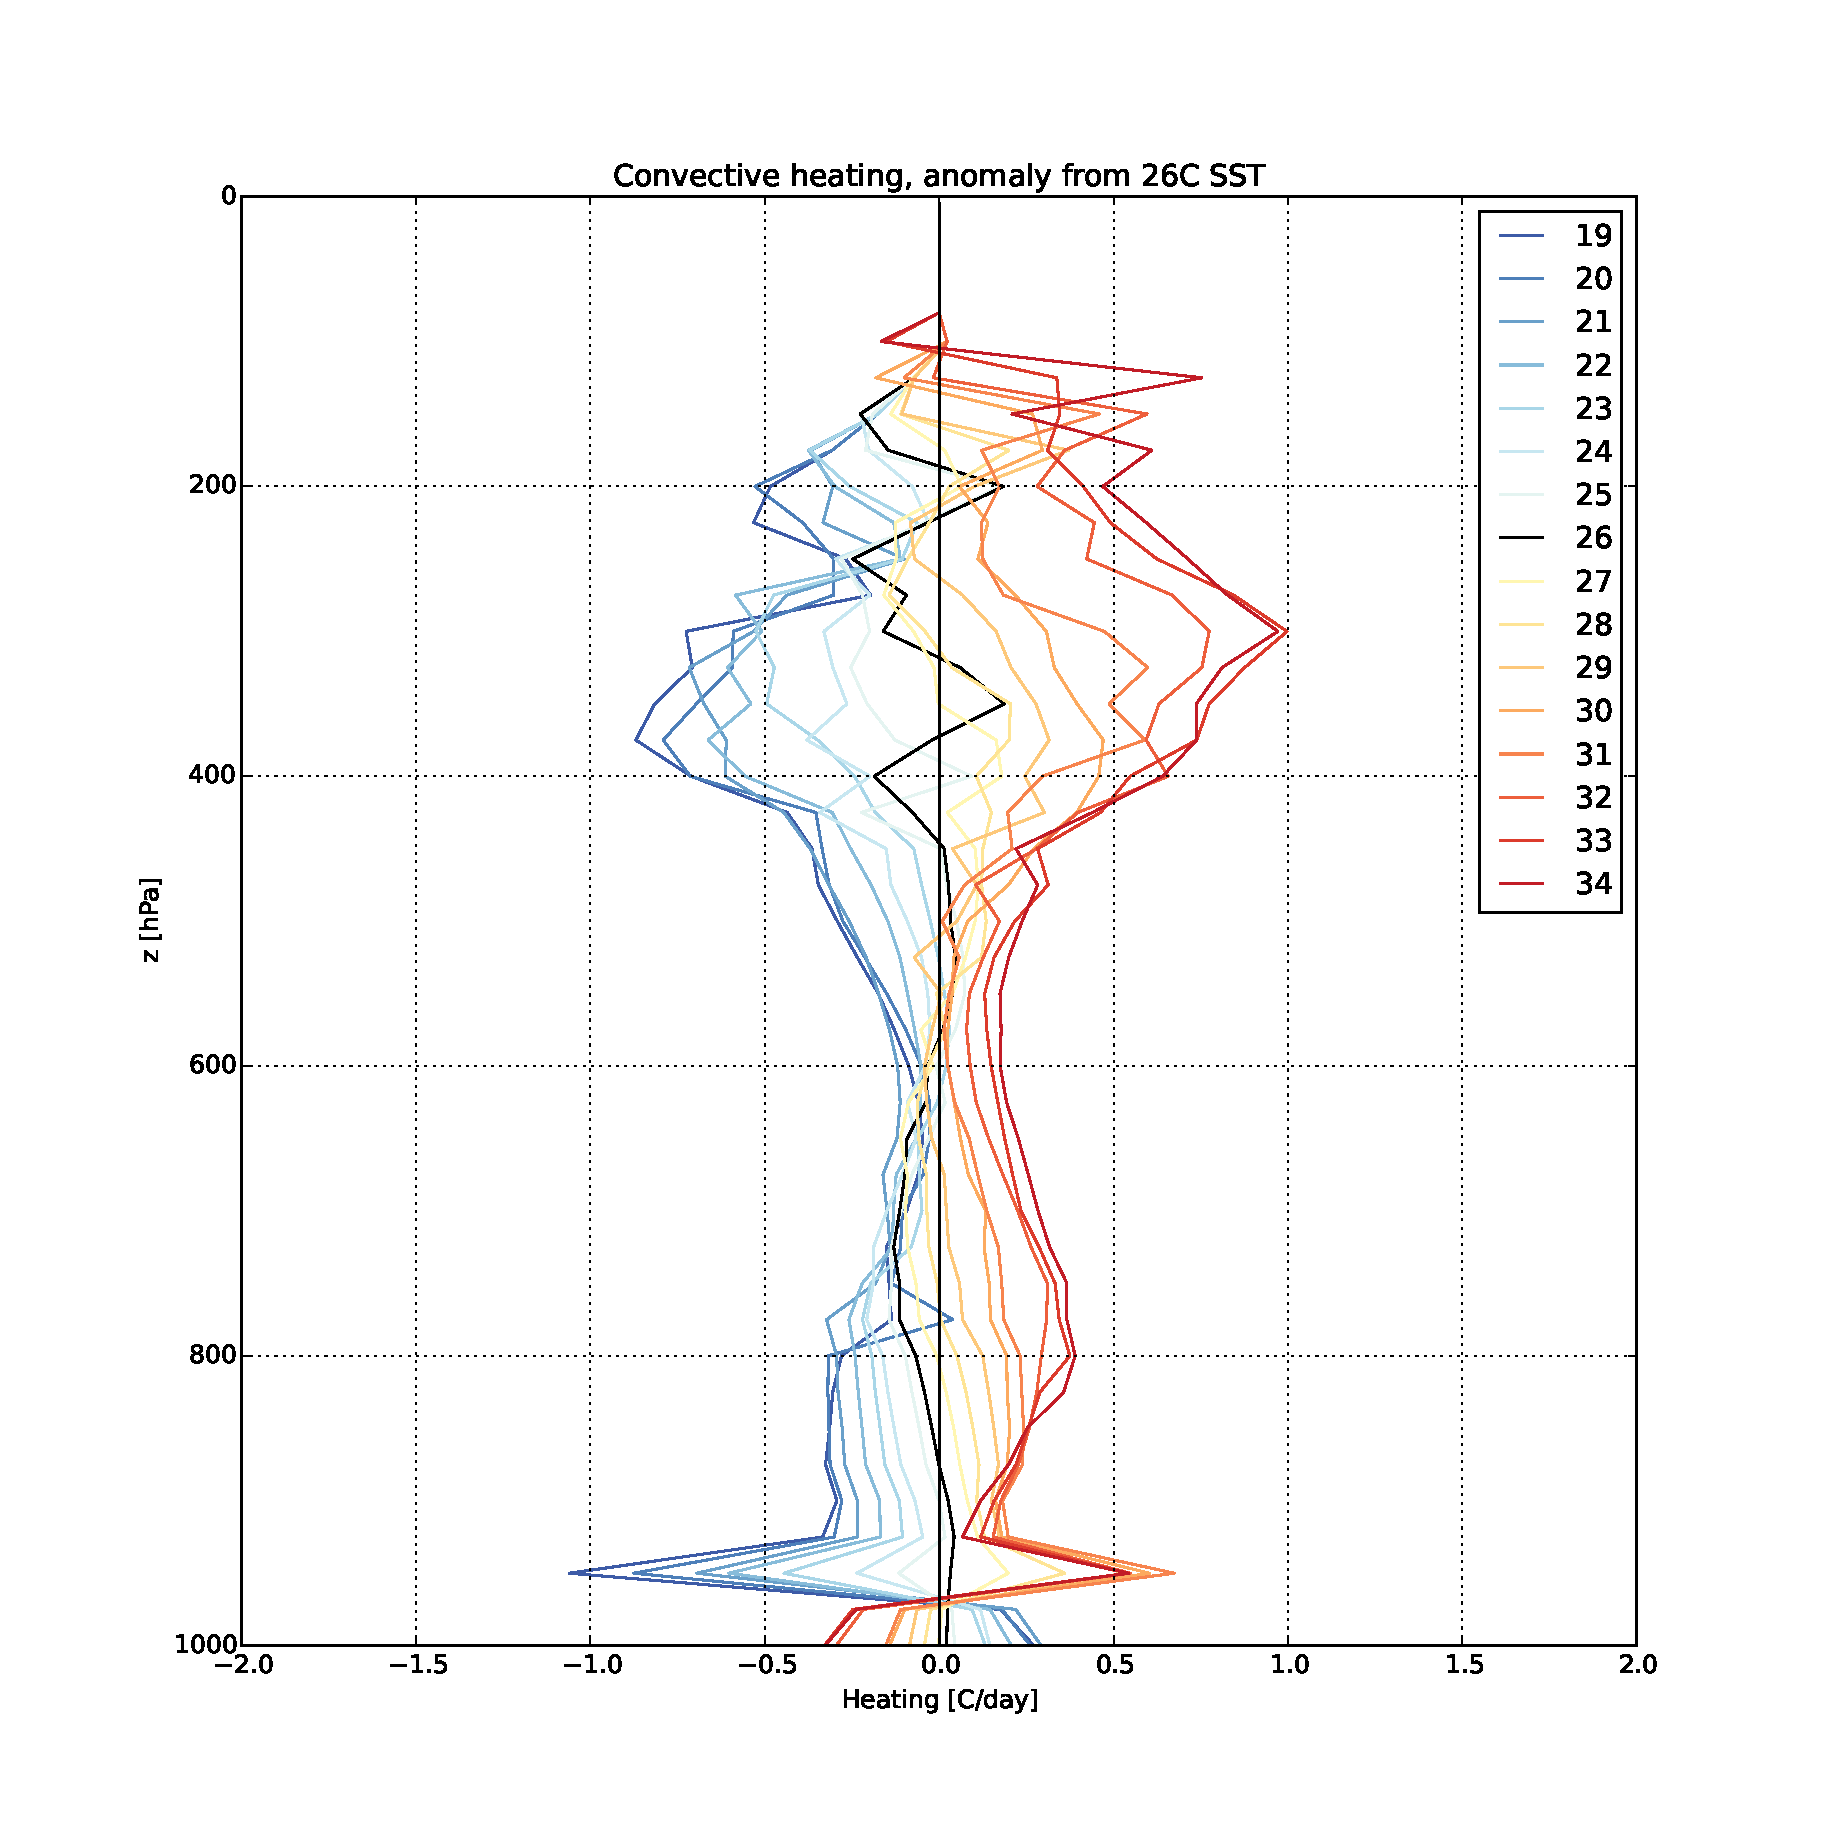
\includegraphics[width=0.3\textwidth]{enso_prof_cq_meananom.eps}
\caption{Heating and temperature profiles for the SCM. a) Temperature anomaly 
relative to \SI{26}{\degreeCelsius}, b) Amplification relative to the mean 
profile c) Moist convective heating rates, anomaly from the mean profile.}
\label{fig:scmsstprof}
\end{figure}

\begin{itemize}
	\item WTG assumption
	\item Generation of atmospheric profiles
	\item Parameter values;
		\begin{itemize}
			\item Land surface - Evaporative fraction
			\item WTG - pressure level of fixed temp profile
			\item Interactive clouds
		\end{itemize}
\end{itemize}
\paragraph{Values of l/s contrast for varying land/tropos parameters}

\begin{center}
	\begin{table}[ht]
		\caption{Land/Ocean contrast in single column model, using WTG over lad 
		surfaces}
		\label{tab:scmphi}
		\scriptsize
	\begin{tabular}{ l  c  c  c }
		\textit{Evap Fraction}		& 0.3   & 0.5  & 0.7 \\ \hline
		\textbf{PFixT 800hPa}\\%\hline
	Phi  							& 1.41  & 1.43 & 1.18\\ %\hline
	Corr.							& 0.57  & 0.78 & 0.64\\ %\hline
	Ratio STD           			& 2.48  & 1.84 & 1.60\\ \hline
		\textbf{PFixT 700hPa}\\%\hline
	Phi  							& 1.39  & 1.30 & 1.15\\ %\hline
	Corr.							& 0.50  & 0.77 & 0.76\\ %\hline
	Ratio STD           			& 2.76  & 1.68 & 1.52\\ \hline
		\textbf{PFixT 600hPa}\\%\hline
	Phi  							& 1.63  & 1.25 & 1.11\\ %\hline
	Corr.							& 0.70  & 0.79 & 0.78\\ %\hline
	Ratio STD           			& 2.35  & 1.58 & 1.42\\ \hline
	\end{tabular}
	\end{table}
\end{center}
\paragraph{Atmospheric profiles}

\begin{figure}[ht]
\includegraphics[width=0.6\textwidth]{{land_thetaprof_e3_p600}.eps}
\includegraphics[width=0.6\textwidth]{{land_deltatheta_e3_p600}.eps}
\caption{Profiles of theta (left), absolute change in theta from median theta 
value (right) - Should show that extreme values (positive and negative) change 
most.}
\label{fig:scmthprof}
\end{figure}

\clearpage
\paragraph{Variability and instability - Role of convection}

\begin{figure}[ht]
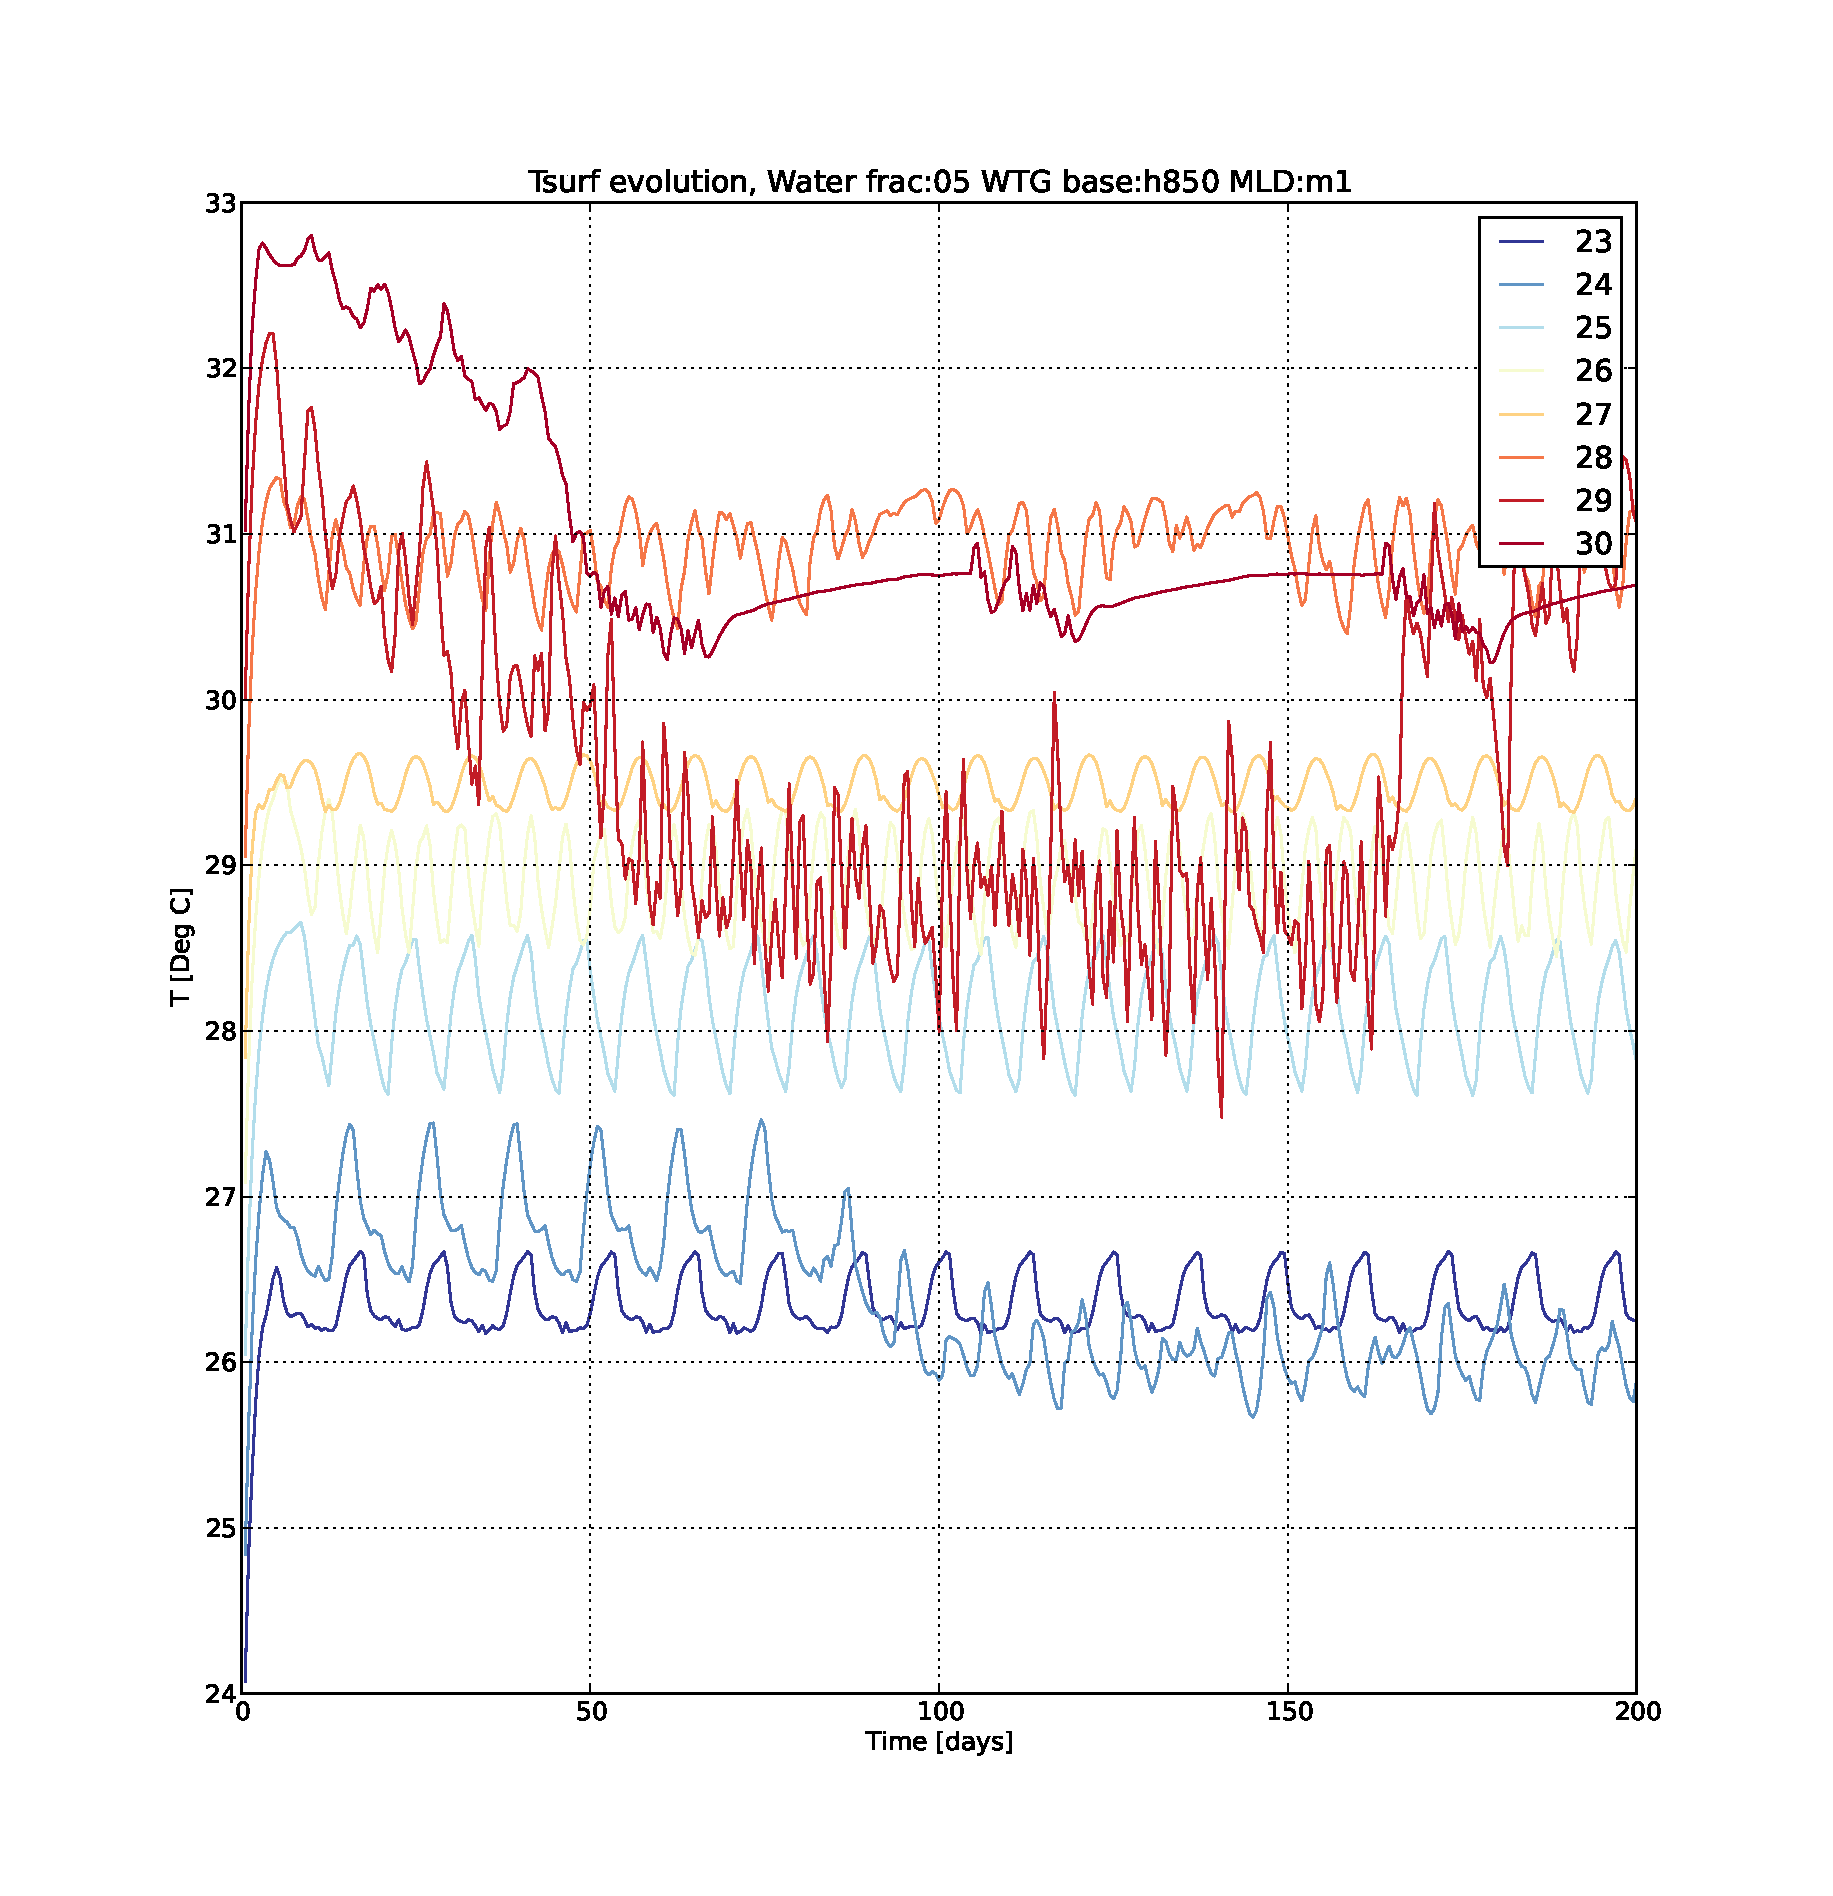
\includegraphics[width=0.5\textwidth]{land_Tsurf_05_m1_h850.eps}
\caption{Timeseries of Tsurf in SCM forced with tropospheric temperature 
profile.}
\label{fig:scmts}
\end{figure}

\begin{figure}[ht]
\includegraphics[width=0.6\textwidth]{{land_anom_intvar_rh_p600}.eps}
\includegraphics[width=0.6\textwidth]{{land_anom_intvar_lw_p600}.eps}
\includegraphics[width=0.6\textwidth]{{land_anom_intvar_sw_p600}.eps}
\includegraphics[width=0.6\textwidth]{{land_anom_intvar_precip_p600}.eps}
\caption{Timeseries of Tsurf in SCM forced with tropospheric temperature 
profile.}
\label{fig:scmts}
\end{figure}



\clearpage
\subsection{Experiments with a Two-Dimensional Model}

\paragraph{explain setup}
\begin{itemize}
	\item Land/Ocean column configurations
	\item Parameter values;
		\begin{itemize}
			\item Land surface - Evaporative fraction
			\item Interactive clouds
		\end{itemize}
\end{itemize}

\subsubsection{Atmospheric profiles in temp, RH, etc}

\begin{figure}[ht]
	\includegraphics[width=0.5\textwidth]{{l3o1_prof_rh_ef0.05_close}.eps}
	\includegraphics[width=0.5\textwidth]{{l3o1_prof_rh_ef0.05}.eps}
	\includegraphics[width=0.5\textwidth]{{l3o1_prof_theta_ef0.05_close}.eps}
	\includegraphics[width=0.5\textwidth]{{l3o1_prof_theta_ef0.05}.eps}
	\caption{Land/sea contrast in TCM}
\label{fig:TCM_prof}
\end{figure}


\clearpage
\subsubsection{Circulation response}
\begin{figure}[ht]
	\includegraphics[width=0.5\textwidth]{{l3o1_omegal_ef0.05_meansst}.eps}
	\includegraphics[width=0.5\textwidth]{{l85co2_psi_ef0.05_meansst}.eps}
	\caption{Circulatoon response, omega, phi}
	\label{fig:TCM_circ}
\end{figure}


\clearpage

\subsubsection{Values of l/s contrast for varying land parameters}
\begin{figure}[ht]
	\includegraphics[width=0.6\textwidth]{{isstcosz}.eps}
	\caption{Land/sea contrast in TCM}
\label{fig:TCM_Rlo}
\end{figure}

\subsubsection{Variability and instability - Role of convection and clouds}
\begin{figure}[ht]
	\includegraphics[width=0.6\textwidth]{{isstcosz_ic}.eps}
	\caption{Land/sea contrast in TCM}
\label{fig:TCM_Rlo}
\end{figure}

\clearpage

\subsection{Comparison of Simplified Models and GCM results}
\begin{figure}[ht]
	\includegraphics[width=0.5\textwidth]{{fsstreg_prof_ocensfc_e0.05}.eps}
	\includegraphics[width=0.5\textwidth]{{l85co2reg_prof_ocensfc_e0.05}.eps}
	\caption{Land/sea contrast in TCM}
\label{fig:TCM_regprof}
\end{figure}

\begin{figure}[ht]
	\includegraphics[width=0.5\textwidth]{{phi_trop_4ysl}.png}
	\includegraphics[width=0.5\textwidth]{{phi_rcm_4ysl}.png}
	\caption{Land/sea contrast in GCM vs TCM}
\label{fig:TCM_GCM_compare}
\end{figure}


\paragraph{Generation of suitable l/s contrast at varying latitudes/evap fraction}
\paragraph{Mapping results}
\paragraph{Differences/Similarities between GCM/RCM}




%----------------------------------------------------------------------------------------
%	Extra-Tropics
%----------------------------------------------------------------------------------------

\section{Extra-Tropical Response}
\begin{itemize}
	\item Relationship between land and ocean very different in extra-tropics.
	\item Discuss Barsugli, Battitsi atmospheric forcing of SST anomalies.
	\item Largest discrepancies between models and observations exist in 
		extra-tropics.
	\item Changes in cloud cover, winds induced by tropical SSTs can impact 
		extra-tropics, i.e. pacemaker and GREB model results.
	\item COWL - COld Ocean, Warm Land theory...
\end{itemize}

%----------------------------------------------------------------------------------------
%	Regional Response / GREB
%----------------------------------------------------------------------------------------

\section{Regional Response}

\begin{itemize}
	\item Lapse rate theory works well in the mean continental response over 
		land.
	\item According to theory it would be expected that dryer regions would have 
		larger response, since difference in humidity is primary driver of the 
		increased variability over land.
	\item We see from regional response that the magnitude of variability is not 
		correlated with the dryness of the land surface.
	\item In addition to thermodynamic changes, tropical SSTs induce changes in 
		cloud cover, energy transport by winds, soil moisture changes.
	\item Regional importance of these discussed...
\end{itemize}


\subsection{GREB Model}

\subsection{Deconstructing the GCM response}
\paragraph{motivation}
\paragraph{Discuss variables used/available}
\paragraph{Response of pacemaker exp.}
\paragraph{Response of amip exp.}


\subsection{Results - Pacemaker}
\subsubsection{u, v winds}

\begin{figure}[ht]
	\includegraphics[width=0.5\textwidth]{{t_surf.v_anom.pos.4ycomp.response}.eps}
	\includegraphics[width=0.5\textwidth]{{t_surf.u_anom.pos.4ycomp.response}.eps}
	\includegraphics[width=0.5\textwidth]{{t_surf.uv_anom.pos.4ycomp.response}.eps}
	\caption{GREB TSurf response }
\label{fig:GREB_ts_uv}
\end{figure}
\clearpage

\subsubsection{Cloud cover}

\begin{figure}[ht]
	\includegraphics[width=0.5\textwidth]{{t_surf.cld.pos.4ycomp.response}.eps}
	\caption{GREB TSurf response }
\label{fig:GREB_ts_cld}
\end{figure}
\clearpage

\subsubsection{Soil Moisture}
\begin{figure}[ht]
	\includegraphics[width=0.5\textwidth]{{t_surf.smc.pos.4ycomp.response}.eps}
	\caption{GREB TSurf response }
\label{fig:GREB_ts_smc}
\end{figure}

\subsubsection{SST}
\begin{figure}[ht]
	\includegraphics[width=0.5\textwidth]{{t_surf.sst_anom.pos.4ycomp.response}.eps}
	\caption{GREB TSurf response }
\label{fig:GREB_ts_sst}
\end{figure}

\subsubsection{Combined response}
\begin{figure}[ht]
	\includegraphics[width=0.5\textwidth]{{t_surf.uv_sst.pos.4ycomp.response}.eps}
	\caption{GREB TSurf response }
\label{fig:GREB_ts_uvsst}
\end{figure}

\begin{figure}[ht]
	\includegraphics[width=0.5\textwidth]{{t_surf.all.pos.4ycomp.response}.eps}
	\includegraphics[width=0.5\textwidth]{{t_surf.all_sst.pos.4ycomp.response}.eps}
	\caption{GREB TSurf response }
\label{fig:GREB_ts_all}
\end{figure}


\subsection{AMIP Experiments}

\paragraph{u, v winds}
\paragraph{Cloud cover}
\paragraph{Soil Moisture}
\paragraph{SST}
\paragraph{Combined response}


